\section{Computational Efficiency}
\label{sec:results:computation}
\makeplotstrue

The computational cost of the centralized and distributed control approaches was evaluated and is presented in \fig{results:compcost}.
The computation times for the distributed controllers assume a parallelized implementation where each sub-controller is executed using a separate processor. 

\ifmakeplots
\begin{figure}
  \centering
  {\large\bfseries Controller Computation Time per Iteration\\}
  \begin{subfigure}{0.75\linewidth}
    % This file was created by matlab2tikz.
%
\definecolor{mycolor1}{rgb}{0.00000,0.44700,0.74100}%
\definecolor{mycolor2}{rgb}{0.85000,0.32500,0.09800}%
\definecolor{mycolor3}{rgb}{0.92900,0.69400,0.12500}%
%
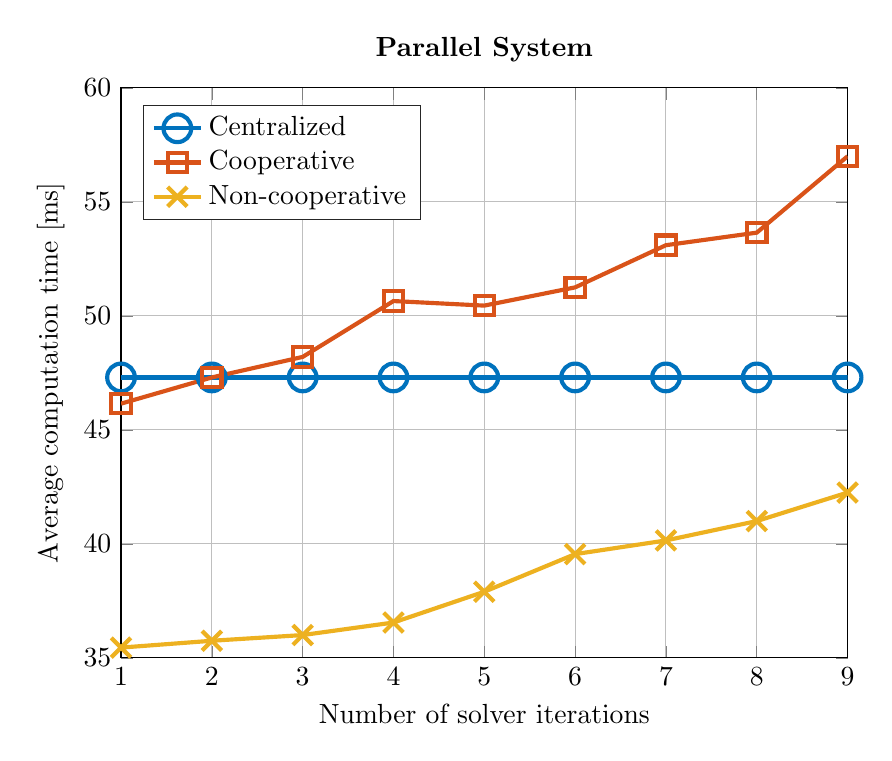
\begin{tikzpicture}

\begin{axis}[%
width=0.761\linewidth,
height=0.597\linewidth,
at={(0\linewidth,0\linewidth)},
scale only axis,
xmin=1,
xmax=9,
xlabel={Number of solver iterations},
xmajorgrids,
ymin=35,
ymax=60,
ylabel={Average computation time [ms]},
ymajorgrids,
axis background/.style={fill=white},
title style={font=\bfseries},
title={Parallel System},
legend style={at={(0.03,0.97)},anchor=north west,legend cell align=left,align=left,draw=white!15!black}
]
\addplot [color=mycolor1,solid,line width=1.5pt,mark size=5.0pt,mark=o,mark options={solid}]
  table[row sep=crcr]{%
1	47.3\\
2	47.3\\
3	47.3\\
4	47.3\\
5	47.3\\
6	47.3\\
7	47.3\\
8	47.3\\
9	47.3\\
};
\addlegendentry{Centralized};

\addplot [color=mycolor2,solid,line width=1.5pt,mark size=3.5pt,mark=square,mark options={solid}]
  table[row sep=crcr]{%
1	46.15\\
2	47.3\\
3	48.2\\
4	50.65\\
5	50.45\\
6	51.25\\
7	53.1\\
8	53.65\\
9	57\\
};
\addlegendentry{Cooperative};

\addplot [color=mycolor3,solid,line width=1.5pt,mark size=5.0pt,mark=x,mark options={solid}]
  table[row sep=crcr]{%
1	35.45\\
2	35.75\\
3	36\\
4	36.55\\
5	37.9\\
6	39.55\\
7	40.15\\
8	41\\
9	42.25\\
};
\addlegendentry{Non-cooperative};

\end{axis}
\end{tikzpicture}%
  \end{subfigure}
  \\
  \begin{subfigure}{0.75\linewidth}
    % This file was created by matlab2tikz.
%
\definecolor{mycolor1}{rgb}{0.00000,0.44700,0.74100}%
\definecolor{mycolor2}{rgb}{0.85000,0.32500,0.09800}%
\definecolor{mycolor3}{rgb}{0.92900,0.69400,0.12500}%
%
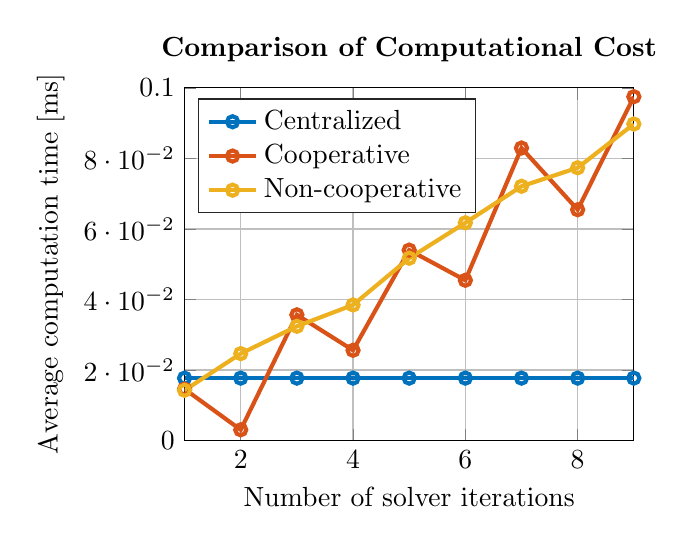
\begin{tikzpicture}

\begin{axis}[%
width=5.706cm,
height=4.479cm,
at={(0cm,0cm)},
scale only axis,
xmin=1,
xmax=9,
xlabel={Number of solver iterations},
xmajorgrids,
ymin=0,
ymax=0.1,
ylabel={Average computation time [ms]},
ymajorgrids,
axis background/.style={fill=white},
title style={font=\bfseries},
title={Comparison of Computational Cost},
legend style={at={(0.03,0.97)},anchor=north west,legend cell align=left,align=left,draw=white!15!black}
]
\addplot [color=mycolor1,solid,line width=1.5pt,mark=o,mark options={solid}]
  table[row sep=crcr]{%
1	0.0177\\
2	0.0177\\
3	0.0177\\
4	0.0177\\
5	0.0177\\
6	0.0177\\
7	0.0177\\
8	0.0177\\
9	0.0177\\
};
\addlegendentry{Centralized};

\addplot [color=mycolor2,solid,line width=1.5pt,mark=o,mark options={solid}]
  table[row sep=crcr]{%
1	0.0146\\
2	0.00305\\
3	0.03565\\
4	0.0256\\
5	0.054\\
6	0.04545\\
7	0.08295\\
8	0.06545\\
9	0.0975\\
};
\addlegendentry{Cooperative};

\addplot [color=mycolor3,solid,line width=1.5pt,mark=o,mark options={solid}]
  table[row sep=crcr]{%
1	0.01425\\
2	0.02465\\
3	0.0324\\
4	0.03845\\
5	0.0517\\
6	0.06175\\
7	0.0721\\
8	0.07735\\
9	0.08975\\
};
\addlegendentry{Non-cooperative};

\end{axis}
\end{tikzpicture}%
  \end{subfigure}
  \caption{Average controller computation time per iteration for centralized and distributed controllers, as a function of the number of solver iterations used. It should be noted that performance gains for solver iterations greater than 2 are marginal. Disturbance (described in \sect{results:performance}) is applied at \u{50}{s} and total simulation time is \u{500}{s}.}
  \label{fig:results:compcost}
\end{figure}

\fi


As expected, the non-cooperative controller achieves the lowest computation times for both the parallel and the serial system.
In both cases, the cooperative controller has a computation time approximately on par with the centralized controller, though slightly lower for few solver iterations.
The computational cost of the cooperative controller relative to the centralized controller is dependent on the operating point: for the parallel system, for example, at the non-disturbed, initial state, a single solver iteration of the cooperative controller requires as much computation time as the centralized controller, but the cooperative controller executes faster at the disturbed operating point.
The number of solver iterations for which the cooperative approach requires more computation time than the centralized approach is thus shifted depending on the simulation case considered.

The computation time for the cooperative controller in the serial case has a zig-zag behavior, where increasing the number of solver iterations from an odd number to an even number actually decreases the computation time.
From \fig{res:qp-compcost}, it is evident that this pattern is a result of the QP solver computation time, however its cause is unclear.

The significant advantage in computation time demonstrated by the non-cooperative controller is a result of the reduced size of its prediction matrices (\giv{prediction-matrices}), which are multiplied as described in \sect{mpc:linearization} to generate the \g{qp}.
The computational cost of the \g{qp} generation is approximately linear in the number of outputs used, and the non-cooperative approach considers fewer outputs than the centralized or cooperative approaches (see \tab{res:parallel-weights}).

For the systems considered here, the QP-generation step has a much higher computational cost than the QP-solving step.
The percentage of computation time spent on solving QPs (including the time required to update the linear QP term after each solver iteration for the distributed controllers) is shown in \fig{res:qp-compcost}.
The remaining time is largely ($>99\%$) dedicated to QP generation.

Using between 2 and 3 solver iterations (for the cases considered, using more iterations has a negligible impact on performance), less than 10\% of the total computation time is spent solving QPs for all control approaches. 
There is thus a limited scope for decreasing the required computation time without decreasing either the number of outputs or states used to generate the QP problem.
Furthermore, the number of outputs used for the cooperative QP is fixed and cannot be decreased, since the sub-controllers have the same cost function, and for the non-cooperative controller only 2 are used so it cannot be further decreased.
Further gains in computational efficiency would therefore require a reduced number of states to be considered when generating the QP problem.

\ifmakeplots
\begin{figure}
  \centering
  {\large\bfseries Computation Time of QP Solver as \% of Total\\}
  \begin{subfigure}{0.75\linewidth}
  % This file was created by matlab2tikz.
%
\definecolor{mycolor1}{rgb}{0.00000,0.44700,0.74100}%
\definecolor{mycolor2}{rgb}{0.85000,0.32500,0.09800}%
\definecolor{mycolor3}{rgb}{0.92900,0.69400,0.12500}%
%
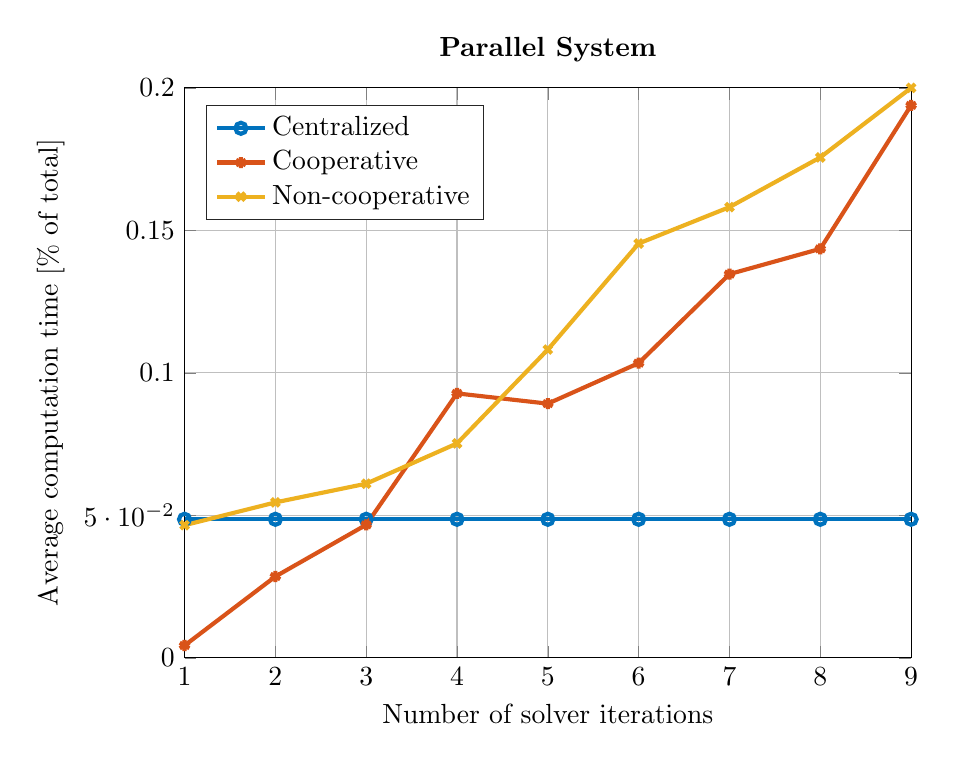
\begin{tikzpicture}

\begin{axis}[%
width=0.761\linewidth,
height=0.597\linewidth,
at={(0\linewidth,0\linewidth)},
scale only axis,
xmin=1,
xmax=9,
xlabel={Number of solver iterations},
xmajorgrids,
ymin=0,
ymax=0.2,
ylabel={Average computation time [\% of total]},
ymajorgrids,
axis background/.style={fill=white},
title style={font=\bfseries},
title={Parallel System},
legend style={at={(0.03,0.97)},anchor=north west,legend cell align=left,align=left,draw=white!15!black}
]
\addplot [color=mycolor1,solid,line width=1.5pt,mark=o,mark options={solid}]
  table[row sep=crcr]{%
1	0.0486257928118393\\
2	0.0486257928118393\\
3	0.0486257928118393\\
4	0.0486257928118393\\
5	0.0486257928118393\\
6	0.0486257928118393\\
7	0.0486257928118393\\
8	0.0486257928118393\\
9	0.0486257928118393\\
};
\addlegendentry{Centralized};

\addplot [color=mycolor2,solid,line width=1.5pt,mark=asterisk,mark options={solid}]
  table[row sep=crcr]{%
1	0.00433369447453957\\
2	0.0285412262156448\\
3	0.0466804979253111\\
4	0.0927936821322803\\
5	0.089197224975223\\
6	0.103414634146341\\
7	0.134651600753296\\
8	0.143522833178006\\
9	0.193859649122807\\
};
\addlegendentry{Cooperative};

\addplot [color=mycolor3,solid,line width=1.5pt,mark=x,mark options={solid}]
  table[row sep=crcr]{%
1	0.0465444287729196\\
2	0.0545454545454546\\
3	0.0611111111111111\\
4	0.0752393980848153\\
5	0.108179419525066\\
6	0.145385587863464\\
7	0.158156911581569\\
8	0.175609756097561\\
9	0.2\\
};
\addlegendentry{Non-cooperative};

\end{axis}
\end{tikzpicture}%
  \end{subfigure}
  \\
  \begin{subfigure}{0.75\linewidth}
  % This file was created by matlab2tikz.
%
\definecolor{mycolor1}{rgb}{0.00000,0.44700,0.74100}%
\definecolor{mycolor2}{rgb}{0.85000,0.32500,0.09800}%
\definecolor{mycolor3}{rgb}{0.92900,0.69400,0.12500}%
%
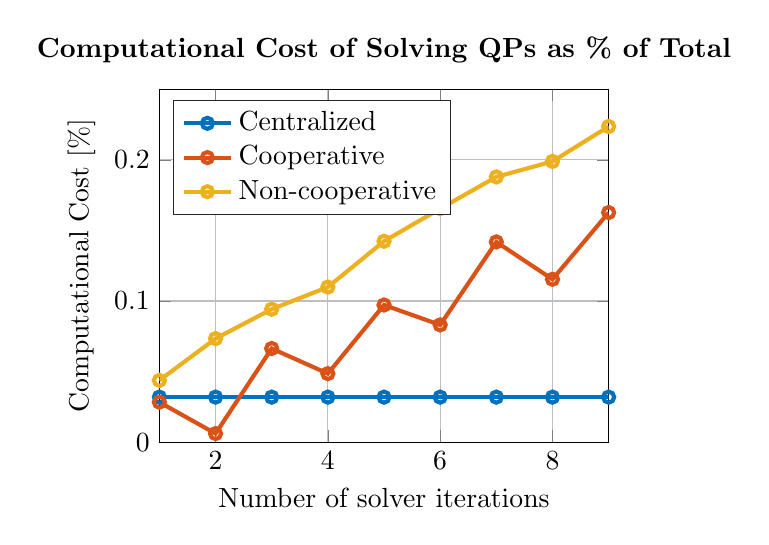
\begin{tikzpicture}

\begin{axis}[%
width=5.706cm,
height=4.479cm,
at={(0cm,0cm)},
scale only axis,
xmin=1,
xmax=9,
xlabel={Number of solver iterations},
xmajorgrids,
ymin=0,
ymax=0.25,
ylabel={Computational Cost [\%]},
ymajorgrids,
axis background/.style={fill=white},
title style={font=\bfseries},
title={Computational Cost of Solving QPs as \% of Total},
legend style={at={(0.03,0.97)},anchor=north west,legend cell align=left,align=left,draw=white!15!black}
]
\addplot [color=mycolor1,solid,line width=1.5pt,mark=o,mark options={solid}]
  table[row sep=crcr]{%
1	0.0318689232985235\\
2	0.0318689232985235\\
3	0.0318689232985235\\
4	0.0318689232985235\\
5	0.0318689232985235\\
6	0.0318689232985235\\
7	0.0318689232985235\\
8	0.0318689232985235\\
9	0.0318689232985235\\
};
\addlegendentry{Centralized};

\addplot [color=mycolor2,solid,line width=1.5pt,mark=o,mark options={solid}]
  table[row sep=crcr]{%
1	0.0282781328684873\\
2	0.0060425953442298\\
3	0.0663440960267981\\
4	0.0485492129717429\\
5	0.097174734569012\\
6	0.0830668006945079\\
7	0.141879757119644\\
8	0.115401569249758\\
9	0.162716955941255\\
};
\addlegendentry{Cooperative};

\addplot [color=mycolor3,solid,line width=1.5pt,mark=o,mark options={solid}]
  table[row sep=crcr]{%
1	0.0437519189438134\\
2	0.0733412674799166\\
3	0.0942271339246764\\
4	0.109888539582738\\
5	0.142365413740878\\
6	0.165460878885316\\
7	0.187980706557163\\
8	0.198945473251029\\
9	0.223703888334995\\
};
\addlegendentry{Non-cooperative};

\end{axis}
\end{tikzpicture}%
  \end{subfigure}
  \caption{Computation time required for QP solver as \% of total controller computation time. Includes time required to update linear term of QP at each solver iteration, as described in \sect{mpc:distributed}. Remaining time is used for generating the initial QP problem. Disturbance (described in \sect{results:performance}) is applied at \u{50}{s} and total simulation time is \u{500}{s}.}
  \label{fig:res:qp-compcost}
\end{figure}
\fi

